% TEMPLATE for Usenix papers, specifically to meet requirements of
%  USENIX '05
% originally a template for producing IEEE-format articles using LaTeX.
%   written by Matthew Ward, CS Department, Worcester Polytechnic Institute.
% adapted by David Beazley for his excellent SWIG paper in Proceedings,
%   Tcl 96
% turned into a smartass generic template by De Clarke, with thanks to
%   both the above pioneers
% use at your own risk.  Complaints to /dev/null.
% make it two column with no page numbering, default is 10 point

% Munged by Fred Douglis <douglis@research.att.com> 10/97 to separate
% the .sty file from the LaTeX source template, so that people can
% more easily include the .sty file into an existing document.  Also
% changed to more closely follow the style guidelines as represented
% by the Word sample file. 

% Note that since 2010, USENIX does not require endnotes. If you want
% foot of page notes, don't include the endnotes package in the 
% usepackage command, below.

% This version uses the latex2e styles, not the very ancient 2.09 stuff.
\documentclass[letterpaper,twocolumn,10pt]{article}
\usepackage{usenix,epsfig,endnotes}
\usepackage{amsmath}
\usepackage{hyperref}
\usepackage{xspace}
\usepackage{tikz}
\usepackage{mdwlist}
\usepackage[font={bf,small}]{caption}
\usepackage{url}
\newcommand{\reminder}[1]{{\textcolor{red}{***#1***}}}
\newcommand{\makeclean}{
    \renewcommand{\reminder}[1]{}
}
\begin{document}

%don't want date printed
\date{April 27, 2015}

%make title bold and 14 pt font (Latex default is non-bold, 16 pt)
\title{\Large \bf Hadoop v1.0 Memory “Failures” Debugger}

%for single author (just remove % characters)
\author{
{\rm San-Chuan Hung}~~~~~{\rm Di Jin}~~~~~{\rm Ye Zhou}\thanks{Authors are listed in alphabetical order}\\
Computational Data Science\\
Carnegie Mellon University\\
\{sanchuah, dijin, yezhou\}@andrew.cmu.edu\\
% copy the following lines to add more authors
} % end author

\maketitle

% Use the following at camera-ready time to suppress page numbers.
% Comment it out when you first submit the paper for review.
\thispagestyle{empty}


\subsection*{Abstract}
\label{sec:dl}

The publication of Google MapReduce and its open-source version, Hadoop, simplify the large-scale data processing procedures and improve the computation efficiency by scheduling a job into multiple tasks running in parallel. 
Tasks with memory consumption exceeding the limit of operating systems are killed and restarted, which might result in both time and memory inefficiency, and this is common for users running their MapRedue programs with the default parameter settings.
To improve this situation, we present a memory failures debugger based on Ganglia to monitor the memory consumption behaviors of Hadoop version 1.2.1 jobs through JMX in a real-time manner. We build a set of MapReduce benchmark jobs to mimic some forms of jobs that might result in exceeding memory consumption and the reschedule of specific tasks. We also develop a parameter recommender, Memtirc, to assist users with tuning of parameters required to avoid memory failures.



\section{Introduction}
Google MapReduce and its open-source version Hadoop provide a simple yet efficient way to handle large-scale data processing based on commodity machines.
Over the years, Hadoop has become the de-facto benchmark\cite{hayashibara2004varphi} where users ”have instantaneous and almost unrestricted access to vast amounts of computational resources”.
Among various design features of this framework, its simple data processing model and ease-of-use allow even naive users who are not aware of the underlying Hadoop infrastructure are able to develop programs, and this might result in "implicit" problems.
\par
The reason these problems are "implicit" is because that users ignoring them will still get their MapReduce programs running and obtain final results, but during this process, many tasks may be rescheduled and restarted due to memory failures which might render execution delay and memory wastes. 
For example, in the Linux environment TaskTrackers monitor tasks based on the following two conditions:  1) The memory usage of a specific task; 2) The total amount of memory usage of multiple tasks. When either of these two conditions is unsatisfied, TaskTracker would kill the running tasks to release memory.
When such failures happen, Hadoop would attempt to rerun these tasks until the number of attempts reaches the configured limit, and then report error messages to users, whose common solution is to modify their code and re-run the program.
\par

The above example is a common scenario where memory failures might occur, and the way that Hadoop handles such failures is simply rescheduling the failed tasks until they successfully finish or aborted, which results in delay in job processing and inappropriate memory usages.
However, this problem can be fixed through parameter tuning in the configuration files provided to the users which is generally ignored, but this solution leads to a question: what parameters to tune and when should we do that? 
We address this problem by describing the design and implementation of a memory usage monitoring system, Memmetric, with the display of specific parameters, therefore users can obtain both the real-time and historical memory usage behaviors of their MapReduce jobs which can be used to illustrate the anonymous memory failures.
For example, if the overall memory usage of a task increases mildly but then decreases greatly in a short period of time, it implies that it is possible that there are some tasks killed and rescheduled by TaskTracker at that time.
By comparing with the historical maximum value of memory used can the user modify the maximum memory allocation for tasks in Hadoop configuration, therefore users can improve their Hadoop program performance without modifying the codes.
\par
The solution of providing both real-time and historical memory usages brings three challenges: 1). How to collect the task-level real-time memory usage metrics from each node in a cluster? 2). How to make sense of the memory usage behaviors and potential memory failures they might lead? 3). How to display the information to users in a straightforward way to help them improve the configuration?
\par
The solutions for these three challenges form three primary components of this paper. For the first challenge, we adopt Ganglia to extract the information of each node for two reasons: i. Ganglia is a real-time monitor that integrates with Hadoop; ii. The rrd adopted by Ganglia can store "fresh" data collected to avoid the overgrowth of database thus guaranteeing performance. A detailed description on Ganglia is in Section 3.
Moreover, the default GangliaSink31 is not suitable for collecting task-level metrics, therefore some existing functions in it should be overwritten.
For the second challenge, we study three types of memory failures: Java heap size error, tasks killed by TaskMemoryManagerThread, and excessive slots.
Based on that, we designed a set of workloads that might lead to memory failures which can happen in real-world Hadoop jobs.
For the third question, the default web frontend displays all the metrics collected by Ganglia which renders it comprehensive but complicated. For the purpose of extracting memory usage from the huge amount of metrics, we provide a web frontend specifically displaying the memory usage metrics.
\par
For the purpose of better understanding the behaviors of memory allocation in Hadoop jobs, we design a set of memory allocation patterns and based on the analysis results from Memmetric we are able to study different memory usage patterns that might result in memory failures, including memory usage patterns under different Hadoop configurations.
\par
The main contributions of this paper include:
\begin{itemize}
	\setlength{\itemsep}{1pt}
	 \setlength{\parskip}{0pt}
	 \setlength{\parsep}{0pt}
	\item
		\emph{ Establishing the monitoring system for task level memory usages for Hadoop 1.2.1.} We adopt Ganglia and construct a monitor providing both real-time and historical memory usage behaviors.
	\item
		\emph{ Detecting several bugs in Hadoop 1.2.1.} When deploying Ganglia, we detect several bugs in Hadoop 1.2.1 which render it unable to provide task-level metrics of each Datanode. We also provide GangliaSink32, a modified version of the default GangliaSink31 to collect task-level memory usage metrics of each node.
	\item
		\emph{ Providing a set of workload behaviors to study the behaviors of memory failures.} We provide a set of workload Hadoop jobs to study three different types of memory failures that might happen in arbitrary Hadoop jobs.
\end{itemize}

The rest of this paper is organized as follows. Section 2 covers detailed explanation of implicit bugs and background materials related to distributed monitoring systems. Section 3 describes the design and implementation of different components of Memmetric. Section 4 describes the experiments, designed workloads and the analysis of the experiment results. Finally, Section 5 covers some experience we learned from this project and the conclusion.




\section{Background}
\subsection{Implicit Bugs}
In this paper, we study three cases of memory failures: Java heap size error, tasks killed by TaskMemoryManagerThread, and excessive slots.
\subsubsection{Java Heap Size Failure}
Without modifying the configuration files Hadoop would run with default setting where most memory-related parameters are set as -1, and in this case only the memory sizes of java virtual machines (JVM) limit the memory that tasks can consume.
The JVM memory consists of three parts as displayed in Figure\ref{ref:heap_structure}.
\par
\begin{figure}[ht]
  \centering
    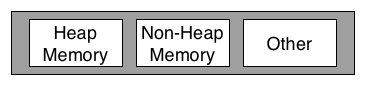
\includegraphics[width=2.7in]{image/Jvm_Heap.png}
    \caption{Java virtual machine memory structure.}
    \label{ref:heap_structure}
\end{figure}
The Heap Memory is the storage for Java objects, which occupies normally the largest part of JVM memory. The default Heap Memory size is 200 MB ({\bf -Xmx200m}) in Hadoop, by modifying this value can users specify memory space allocated to tasks.
In the runtime the total memory usage of the JVM may exceed the value specified in the command after "{\bf -Xmx}", this is because of the non-heap memory and other storage in JVM memory.
The Non-Heap Memory  is created at the JVM startup and store structures such as runtime constants, method data, the code for methods and constructors, and interned Strings.
There are also some other parts that might consume memory including JVM code itself, JVM internal structures, loaded profiler agent code and data, etc, which normally occupie a small portion of total JVM memory. 

\subsubsection{TaskMemoryManagerThread}
In addition to the execution of tasks, Hadoop also monitors these tasks and provides metrics reflecting their status for the purpose of rescheduling the killed ones.
In the Linux environment, TaskTrackers monitor tasks based on the following two conditions:  1) The memory usage of a specific task; 2) The total amount of memory usage of multiple tasks.
In the former situation, a task is killed and rescheduled by the TaskTracker if it fails either of the following two criteria:
i. Anytime when the current memory usage of a task exceeds two times of the value specified by {\bf mapred.cluster.max.map.memory.mb};
ii. The current memory usage of a task exceeds the value specified by {\bf mapred.cluster.max.map.memory.mb} for two consecutive periods of time (default is 5s). 
The first criteria considers the operation of fork(), which results in duplicated memory usages; the second criteria is applied to avoid the appearance of stragglers.
In the latter situation, tasks are killed by the TaskTracker if the following criteria is satisfied:
\begin{equation}
{\emph memInUsage} > {\emph maxMemAllowedForAllTasks} 
\end{equation}
where \emph {memInUsage} denotes the total memory in use of all the tasks scheduled by a specific TaskTracker and \emph {maxMemAllowedForAllTasks} denotes the total amount of memory allocated to it. The latter parameter can be calculated as following:
\begin{equation*}
\begin{aligned}
&{\emph maxMemAllowedForAllTasks} = \\
& \hspace {5pt} {\emph maxCurrMapTasks} \times {\emph mapSlotMemSizeOnTT} + \\
& \hspace {5pt} {\emph maxCurrReduceTasks} \times {\emph reduceSlotSizeMemOnTT}
\end{aligned}
\end{equation*}
In the above equation, \emph {maxCurrMapTasks} (specified by {\bf mapred.tasktracker.map.tasks.maximum} in the code) denotes the number of map slots allocated to that TaskTracker and \emph {mapSlotMemSizeOnTT}, which is specified by {\bf mapred.cluster.map.memory.mb}, denotes the memory size of a map slot. 
For reduce tasks, the situations are similar except that the parameters applied are different.
All tasks are killed by TaskTracker in the reverse order of scheduled time, \emph{i.e.}, recent tasks are killed until equation (1) fails. 
\subsubsection{Excessive Slots}
There is another case when Hadoop jobs may encounter memory failures: the virtual memory allocation request is under the limit specified by JVM, but the total value exceeds the amount of actual physical memory in the machine where TaskTracker is running.
This case can happen due to inappropriate settings on the number of slots (default value is 2) allocated to the TaskTracker. Consider the case illustrated in Figure \ref{ref:excessive_slots}.
\begin{figure}[ht]
  \centering
    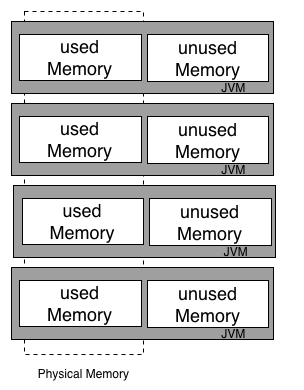
\includegraphics[width=2.1in]{image/excessive_Slots.png}
    \caption{Excessive number of slots}
    \label{ref:excessive_slots}
\end{figure}
\par
Suppose the physical memory space is 800 MB, the JVM heap size is 300 MB and one TaskTracker is allocated with 4 slots. Hadoop would run smoothly if the total memory consumed in the four JVMs is under 800 MB, but once the total amount of memory consumed exceeds the physical memory space, errors would occur and Hadoop would have to kill the running tasks to reduce the amount of memory occupied, or just abort the whole process.
\par
With appropriate parameters tuning, users can better manage the memory consumed by tasks, and the JVM memory space can be fully utilized to avoid potential memory-related bugs existing in users' Hadoop programs.

\subsection{Related Work}
Even though Hadoop has its own monitoring system on each component, including the website on JobTracker to check the running status of each MapReduce job and the website on the Namenode to check the usage of Hadoop File System (HDFS), the information posted on these pages is always not enough for either naive or experienced users.
For naive users, they merely get the log description showing the failed status of their jobs without specific reasons; For experienced users who need to know more about the whole pipeline performance information involved with a bunch of jobs, the default monitoring system is not enough either.
With the popularity of complex pipeline MapReduce jobs, companies like LinkedIn, Hortonworks develop their own fine-grained monitor frameworks for Hadoop based on traditional monitoring frameworks for cluster nodes metrics.\par
Ganglia\cite{massie2004ganglia}, developed from the project named Millennium in UC Berkeley, is a scalable distributed monitoring tool for high performance computing systems, which naturally integrates with Hadoop.
Ganglia follows the master/slave infrastructure, running a Ganglia monitoring daemon (Gmond) on each node in the cluster that needs to be monitored.
Gmond collects metric information on this node such as metrics of CPU,memory, etc, and sends it to Ganglia Meta Daemon (Gmetad) running on the master monitoring node of the cluster via XML over TCP periodically.
The Gmetad process runs on the master monitoring node (may not be the master of a cluster) to collect the metrics from distributed Gmond processes and Ganglia has its own default PHP web front end to show these metrics with dashboards.
%Gmond is a multi-threaded daemon which monitors changes in host state, announce the metrics data in Unicasting or Multicasting way. Hadoop has support of integration with Ganglia


Nagios (Nagios Ain’t Goona Insist On Saintood) \cite{josephsen2007building} is an open-source monitoring system that has great freedom and flexibility. 
The core of Nagios is concise, but it can be extended with specific plug-ins for different requirements, including plug-ins implemented by the developers.
These plug-ins run on distributed nodes to monitor the their status and send metrics to the core. 
The advantages of Nagios is that it provides a bunch of alerts mechanism that can notify the administrator when there is a problem in the system.
\par
Chukwa\cite{boulon2008chukwa} is a subproject of Hadoop, which is a distributed log analysis monitoring system. 
Different with Ganglia or Nagios, which are real-time monitoring systems, Chukwa is a batch log analysis system with the ability of processing large data brought by Hadoop.
Chukwa provides a full stack solution for large scale log data including data collection, storage, analysis and dashboard display.
Chukwa also deploys an agent running on each node to monitor metrics status on that node and the "Chukwa Collector" takes responsibility to collect these metrics data from distributed agents. 
After classifying, sorting, de-duplicating and combining, those logs will be directly written to HDFS or HBase which can be used as the input source for MapReduce analysis jobs, then the results of the analysis are displayed through websites.
Users can check the running status of MapReduce jobs including the running time, resource consumption, when the failure happens and where the bottleneck is of the whole pipeline which largely enriches the monitoring functionality.
\par
SequenceIQ\cite{http://sequenceiq.com} is a real-time distributed monitoring system built directly atop InfluxDB and Grafana which provides comprehensive analysis on various metrics such as CPU, memory, network usage, etc..
InfluxDB\cite{http://influxdb.com} is a time series, metrics and analytics distributed database that can be used as part of the monitoring system due to its specific design for storing metrics data and support for abundant SQL query for analysis.
Each node in the cluster can insert metrics data into InfluxDB, users do not need to care about the distributed message and data transferring; instead they just need to use database functions to update the metrics.
Grafana\cite{http://grafana.org} is a well-designed and easy-to-use website development tool which integrates dashboards with analytics. Grafana provides rich graphing, mixed styling which render it a powerful frontend analysis tool.
\par

Cloudera Manager\cite{http://www.cloudera.com} is the first and most sophisticated commercial management application for Hadoop clusters in the industry. 
It is designed to make the administration of enterprise data hub at any scale simple and straightforward, which provides users cluster-wide, real-time views of nodes/jobs running status, incorporating a full range of reporting and diagnostic tools to help user optimize performance.

Ambri\cite{http://hortonworks.com/hadoop/ambari} developed by Hortonworks is an open-source version of Cloudera Manager which can be used to monitor the status of Hadoop jobs.
Ambri adopts Ganglia to collect metrics and Nagios to support the alert system, based on which users can check the status of Hadoop core as well as HBase and Hive.
For the purpose of integrating with existing administration tools, Ambri exposes the monitoring metrics through RESTful API.
\par
White Elephant\cite{http://data.linkedin.com/opensource/white-elephant}, developed by LinkedIn, is an open sourced Hadoop log aggregating tool and dashboard which enables visualization of Hadoop cluster utilization across users. 
White Elephant runs a daemon on each node in the cluster to periodically collect the log data, then it runs a sequence of MapReduce jobs to compute aggregate statistics. In the end, White Elephant applies a viewer application to display the metrics with dashboard.
\par
The difference between our system and Chukwa and White Elephant is that we use real-time metrics collected from Ganglia instead of the logs in each node.
Unlike Cloudera Manager, Ambri, and White Elephant which provide a general monitoring system, our system focuses on memory by providing fine-grained monitoring on task level and event detection for memory usages. It also provides the parameter description for users to modify to improve the performance of their Hadoop programs.




\section{System Architecture}
\begin{figure*}[ht]
  \centering
    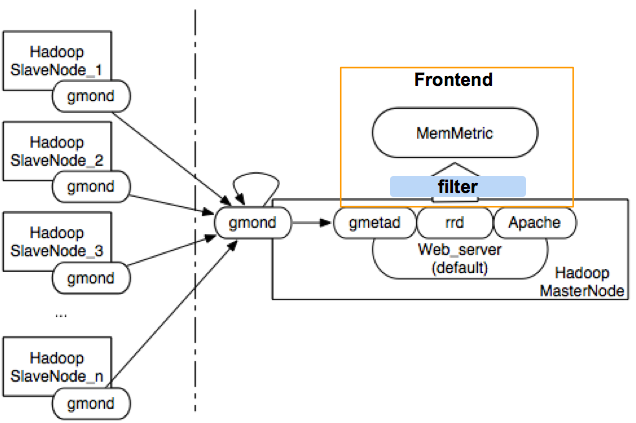
\includegraphics[width=4.0in]{image/architecture.png}
    \caption{System Architecture}
    \label{ref:architecture}
\end{figure*}

Figure \ref{ref:architecture} shows our system design. It contains three main components: \textbf{Ganglia}, \textbf{Hadoop metric system}, and \textbf{Memmetric}. We used Ganglia 3.6.0 as the infrastructure to gather the  Hadoop cluster metrics in real-time. Each node in the Hadoop cluster periodically reports its information to Ganglia daemon. After Ganglia collecting the metric information, it will be organized and visualized to users through the frontend of Memmetric.

\subsection{Ganglia}

Ganglia deploys a daemon on each node in the cluster called Gmond. Gmond in a worker node is responsible for collecting monitoring statistics of a machine (\emph{e.g.}, CPU load, memory usage, disk load), and reporting these metrics to the Gmond on the master node. 

Other programs can also send their metrics to the Gmond in the same machine, and then the metrics will be aggregated by Ganglia system. In Memmetric, we deploy Hadoop cluster to send JVM metric which includes task level memory usage information to Gmond.

Gmetad polls the metrics from the Gmond on the master node, and stores the information into round robin database (rrd) periodically. In addition, Ganglia periodically compasses old metric values in rrd, thus avoiding rrd wasting too much disk space to store less-used or antiquated metrics.

Ganglia provides a web interface called ganglia-web, which can plots the metrics in rrds in the form of charts or json. Memmetric queries ganglia-web for the information we needed, organizes them, and visualizes these information. 

\subsubsection{Ganglia Filter}

\begin{figure}[ht]
  \centering
    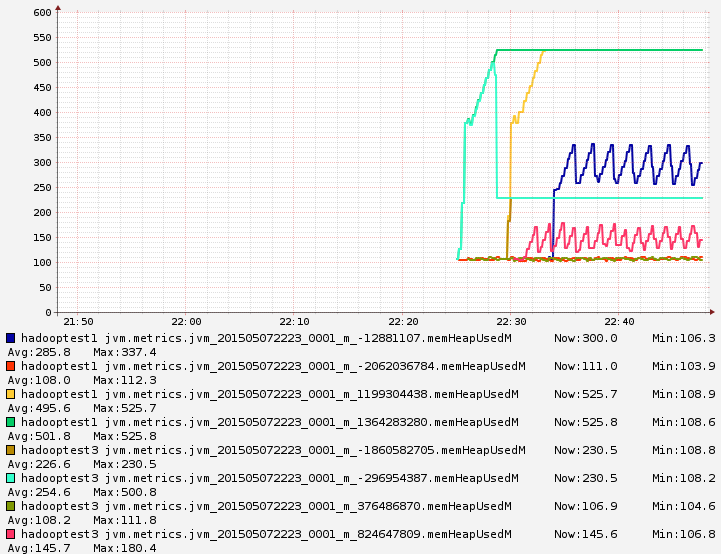
\includegraphics[width=3.0in]{image/ganglia_finished_tasks.png}
    \caption{Ganglia does not set the value of finished tasks as zero}
    \label{ref:gangliah_bug}
\end{figure}

During the process of the deployment of Memmetric, we find that Ganglia keeps reporting finished tasks' metrics as the last values it receives because that Ganglia does not discard received metrics automatically. For example, Figure \ref{ref:gangliah_bug} shows the heap memory usage of tasks in a regular Hadoop job. Presumably, there should be only four map tasks running after 22:35 because we set two map task slots for a machine; however, it turns out that there are six lines of memory usage, one of them, jvm.metrics.jvm\_201505072223\_0001\_m\_-296954387.memHeapUsedM displayed in light blue line finishes at 22:29, but the metric value remains.

This behavior in Ganglia renders the reported memory usage in a machine unreasonably large because the finished task memory usages are all counted into the sum of total memory usage. One solution to this problem is to tune the parameter "delete time" d\_max: When metric is not sent to Ganglia over d\_max time, Ganglia will assume the metric is dead and discard it. However, the value of discarded metrics is not set as zero, but it becomes invisible from Ganglia web-interface, which means that our frontend cannot plot any metrics before d\_max and cannot provide history memory usage information to users. It becomes a dilemma: if d\_max is set to a small number, the finished task metric will be discarded and it will not be counted into the sum of memory usage, but it becomes invisible from the frontend. If d\_max is a large number, the finished task information can retain for longer time, but its value is not set to zero and confuses the sum of total memory usage.

Instead of modifying d\_max, we added a filter inside the Ganglia API server to clean the metrics of finished tasks. If one metric is continual reported as same value over a tolerated period $T$ from time t\_end, the filter will assume the task finishes at t\_end and set the value of the metric after t\_end. 

\subsection{Hadoop Metric System}

Hadoop 1.2.1 already provides metric system to gather different metrics source (e.g., JVM metrics, Remote Procedure Call metrics) in Hadoop cluster and send them to the assigned destination (e.g., files or Ganglia daemon), shown in Figure \ref{fig:metric2}.

\begin{figure}[h!]
  \centering
    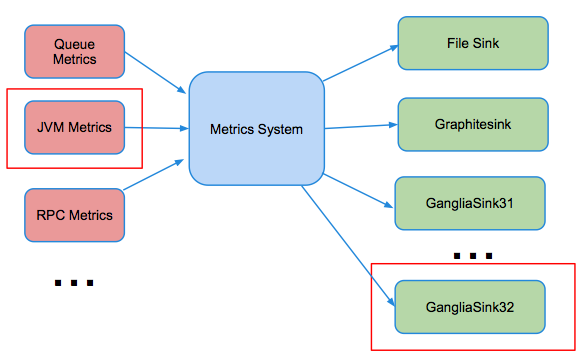
\includegraphics[width=0.5\textwidth]{image/ganglia32}
  \caption{Metric System in Hadoop (Metric2)}
  \label{fig:metric2}
\end{figure}

In our system, we connected "JVM metrics" to metric system, and assigned them sending to Ganglia by GangliaSink. Therefore, Ganglia can receive task level memory usage information from Hadoop metric system.

We found that the default connector between metric system and Ganglia (GangliaSink31.java) behaves unexpectedly; therefore, we revised it to GangliaSink32 to monitor task level information, which is discussed in next section.

\subsubsection{Revised GangliaSink: GangliaSink32}

Each JVM in Hadoop cluster periodically reports it memory usage information into metric system as a key-value pair. The key format is jvm.metric.\{tag\}.heapMemoryUsedM. For example, jvm.metric.jvm\_20140405\_1\_m\_1.heapMemoryUsedM means the heap memory usage of the map task for Hadoop job 20140405\_1. 

However, the original connector between metric system and Ganglia, GangliaSink31.java, will discard the tag of the reported metric key. For example, jvm.metric.jvm\_20140405\_0001\_m\_1.heapMemoryUsedM will become jvm.metric.heapMemoryUsedM. 

\begin{figure}[h!]
  \centering
    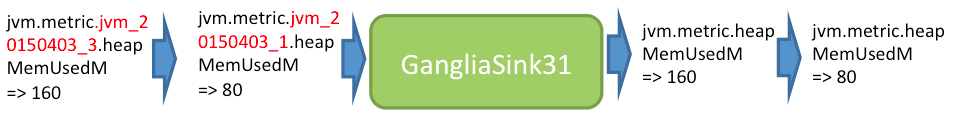
\includegraphics[width=0.5\textwidth]{image/ganglia31_flow.png}
  \caption{GangliaSink31 removes the tag in the key of metric and cause ambiguity.}
\end{figure}

Removing the tag results in that the system cannot discriminate metrics from different running tasks. Therefore, the meaning of jvm.metric.heapMemoryUsedM becomes hard to explain, because we cannot know which target's memory usage does  jvm.metric.heapMemoryUsedM stands for. Also, the system cannot aggregate all task memory usage into a machine aspect memory usage, because they are all mixed in a metric. 

To solve this problem, we developed GangliaSink32.java to replace GangliaSink31.java. GangliaSink32.java can retain the tag of the metric key. Therefore, Ganglia can separate the memory usage information among different processes. 

\begin{figure}[h!]
  \centering
  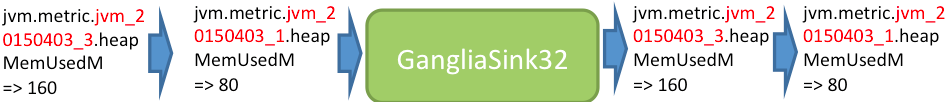
\includegraphics[width=0.5\textwidth]{image/ganglia32_flow.png}
  \caption{GangliaSink32 retains the tag in the key of metric.}
\end{figure}

\subsubsection{Reporting Frequency}

Ganglia can configure the reporting frequency of gmond.  In default, gmond reports in 10 seconds. However, some small map tasks can run in less than 10 seconds, which cannot be observed because it ends before gmond starts to collect memory usage metrics. 
We assigned reporting frequency as 2 seconds to detect fast tasks.

\subsection{Frontend: Memmetric}
We designed our frontend system (Memmetric) in two parts: \textbf{real-time monitor} and \textbf{historical monitor}. Real-time monitor  presents users the current status of the clusters. Historical monitor records anomalous data points to hint users debug their cluster.

\subsubsection{Real-time Monitor}

\begin{figure}[h!]
  \centering
    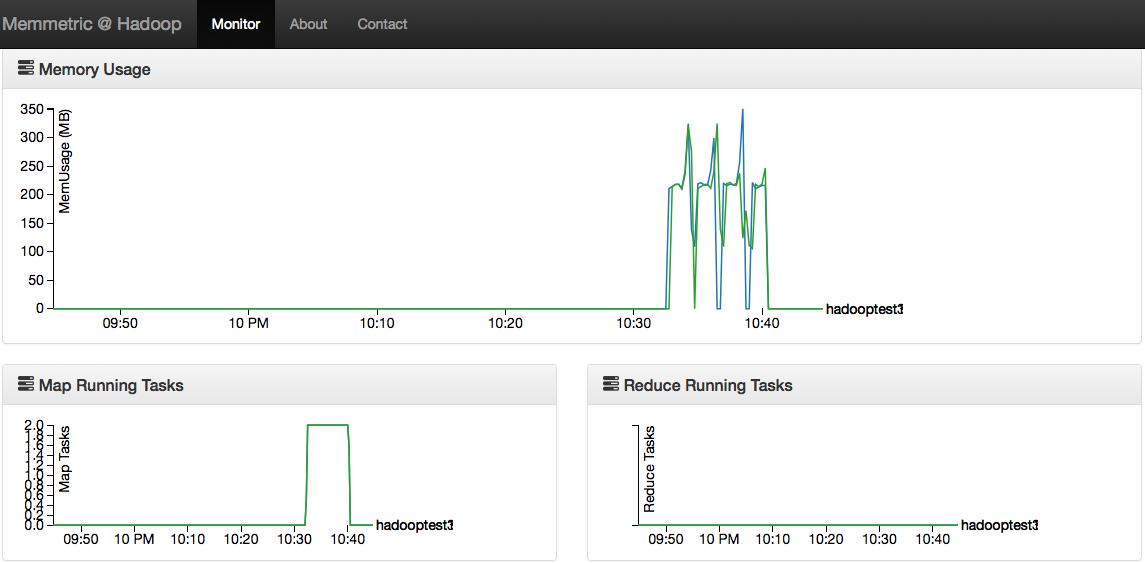
\includegraphics[width=0.5\textwidth]{image/real-time-monitor.png}
  \caption{Real-time Monitor}
\end{figure}

Real-time monitor shows per-machine view of task heap memory usage, the number of running map tasks and reduce tasks. Each line in "Memory Usage" block shows the total heap memory usage in a machine. Also, lines in "Map Running Tasks" and "Reduce Running Tasks" show the number of map an reduce tasks in different machines.

Hadoop cluster reports the memory usage for each task to Ganglia. However, plotting the memory usage of all tasks individually on the same chart can be hard to understand, because a Hadoop job may spawn hundreds of tasks. Therefore, Memmetric aggregates all per-task heap memory usage (jvm.metrics.jvm\_\{process\_id and task type\}.memHeapUsedM) on a machine into a per-machine heap memory usage line. Also, Memmetric shows the number of running map tasks and reduce tasks. Real-time monitor provides a clue whether there are tasks killed due to over memory usage. If there is a sharp drop of heap memory usage on machine, it is possible that some tasks use too many memory to be killed by JVM or operating system. 

\subsubsection{Historical Monitor}

\begin{figure}[h!]
  \centering
    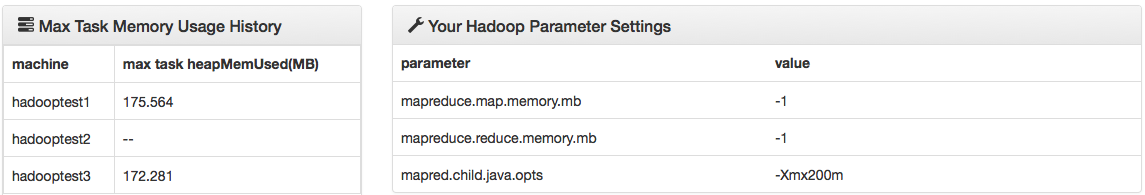
\includegraphics[width=0.5\textwidth]{image/historical-monitor.png}
  \caption{Historical Monitor and Parameter Settings}
\end{figure}

Historical monitor presents the odd data points in each machine for users to revise their cluster parameter settings. Memmetric records the data points of largest task heap memory usage in each machine, because those points are the possible moments where a task violates the memory upper bound restriction and results in failure. For example, if Hadoop cluster sets "mapred.child.java.opt" as "-Xmx200m", which means that  the JVM child of a task at most allocate 200MB memory. If the historical monitor shows that some task has used more than 200MB, it is highly possible that the task will be killed, and the user should consider to modify the parameter to enlarge the maximum heap memory usage.

Besides, Memmetric crawls the configure files in Hadoop directory (i.e. "hadoop/conf") to fetch the parameter settings, and shows them nearby historical monitor. Users can revise their cluster's settings by comparing historical monitor and parameter settings. 

\begin{figure}[h!]
  \centering
    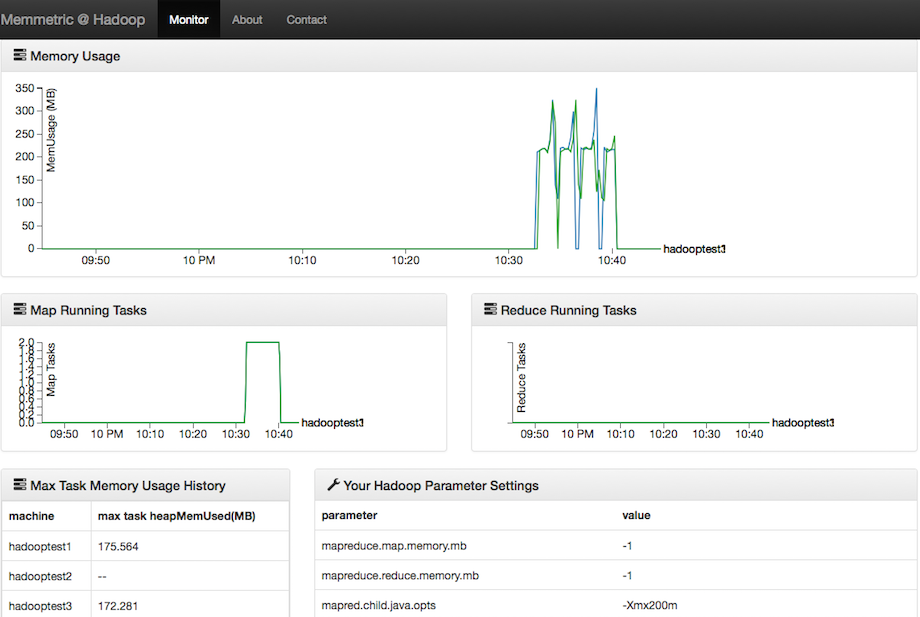
\includegraphics[width=0.5\textwidth]{image/overview.png}
  \caption{Memmetric Overview}
\end{figure}



%\section{Implementation}
%\subsection{GangaliaSink32}

\begin{figure}[h!]
  \caption{Metric2}
  \centering
    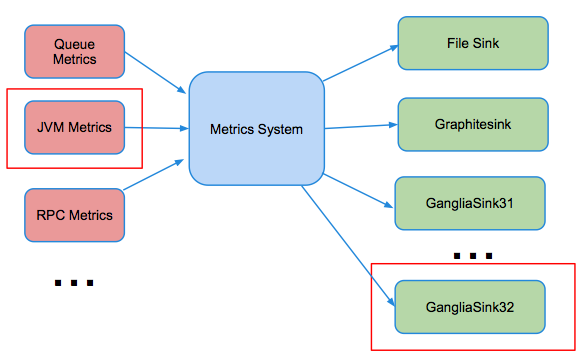
\includegraphics[width=0.5\textwidth]{image/ganglia32}
\end{figure}

\subsection{Ganglia Filter}

We found that Ganglia keeps to report finished task's metric as the last value it received. It makes the reported memory usage in a machine incredible large because the finished task memory usages are all counted into the sum of memory usage.

We added a filter inside the Ganglia API server to clean out the metrics of finished tasks. If one metric is continual reported as same value over tolerated period $T$, the filter will assume the task has finished, and remove the finished metric from reported API. 


%\section{Frontend Design}
%We designed the frontend, called as Memmetric, in two aspects: \textbf{real-time monitor} and \textbf{historical monitor}. Real-time monitor  presents users the current status of the clusters. Historical monitor records anomalous data points to hint users debug their cluster.

\subsection{Real-time Monitor}

\begin{figure}[h!]
  \caption{Real-time Monitor}
  \centering
    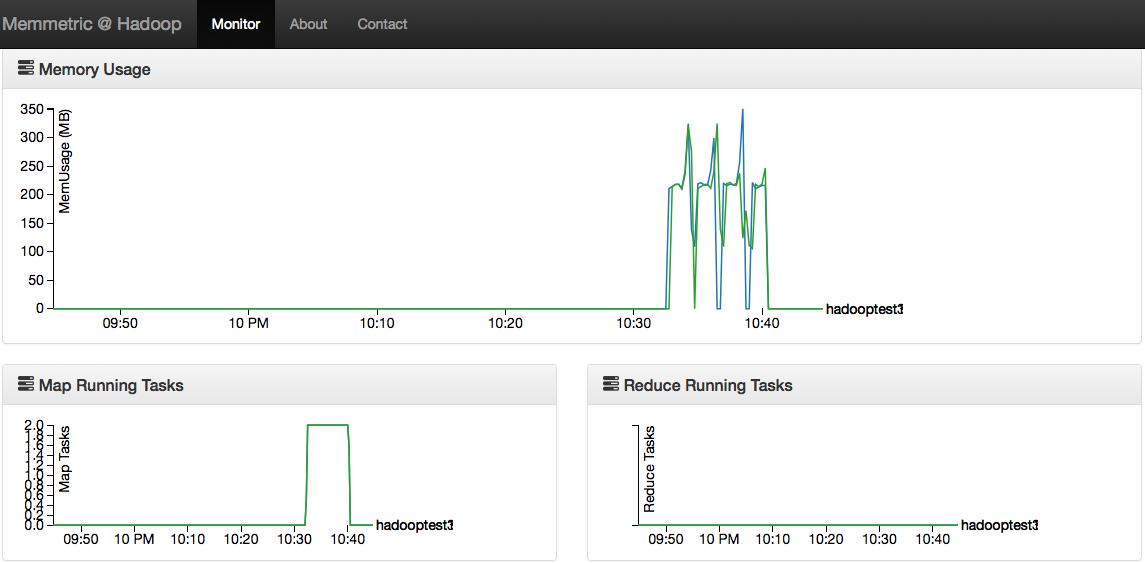
\includegraphics[width=0.5\textwidth]{image/real-time-monitor.png}
\end{figure}

Real-time monitor shows per-machine view of task heap memory usage, the number of running map tasks and reduce tasks. Each line in "Memory Usage" block shows the total heap memory usage in a machine. Also, lines in "Map Running Tasks" and "Reduce Running Tasks" show the number of map an reduce tasks in different machines.

Hadoop cluster reports the memory usage for each task to Ganglia. However, plotting the memory usage of all tasks individually on the same chart can be hard to understand, because a Hadoop job may spawn hundreds of tasks. Therefore, Memmetric aggregates all per-task heap memory usage on a machine into a per-machine heap memory usage line. Also, Memmetric shows the number of running map tasks and reduce tasks. Real-time monitor provides a clue whether there are tasks killed due to over memory usage. If there is a sharp drop of heap memory usage on machine, it is possible that some tasks use too many memory to be killed by JVM or operating system. 

\subsection{Historical Monitor}

\begin{figure}[h!]
  \caption{Historical Monitor and Parameter Settings}
  \centering
    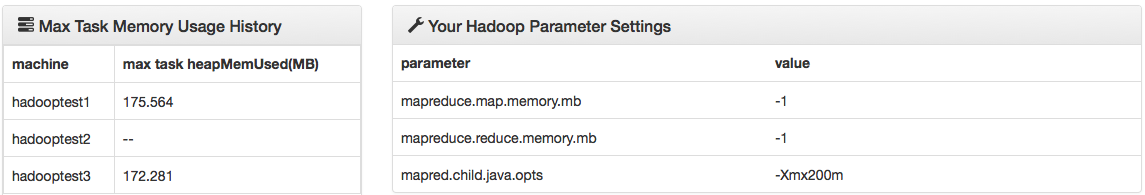
\includegraphics[width=0.5\textwidth]{image/historical-monitor.png}
\end{figure}

Historical monitor presents the odd data points in each machine for users to revise their cluster parameter settings. Memmetric records the data points of largest task heap memory usage in each machine, because those points are the possible moments where a task violates the memory upper bound restriction and results in failure. For example, if Hadoop cluster sets "mapred.child.java.opt" as "-Xmx200m", which means that  the JVM child of a task at most allocate 200MB memory. If the historical monitor shows that some task has used more than 200MB, it is highly possible that the task will be killed, and the user should consider to modify the parameter to enlarge the maximum heap memory usage.

Besides, Memmetric crawls the configure files in Hadoop directory (i.e. "hadoop/conf") to fetch the parameter settings, and shows them nearby historical monitor. Users can revise their cluster's settings by comparing historical monitor and parameter settings. 

\begin{figure}[h!]
  \caption{Memmetric Overview}
  \centering
    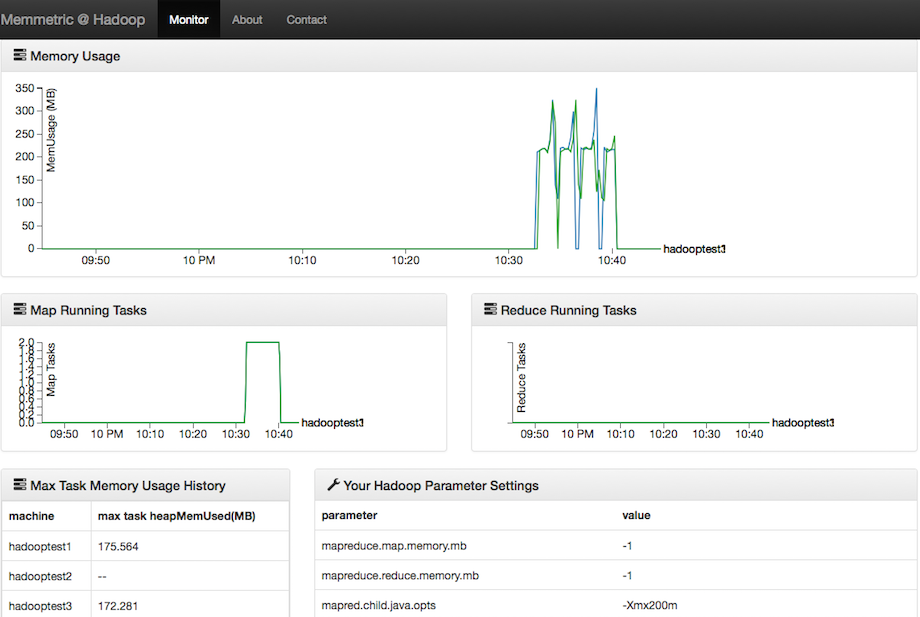
\includegraphics[width=0.5\textwidth]{image/overview.png}
\end{figure}

\section{Evaluation}
\subsection{Customized Memory Behavior WordCount}
To test our Hadoop memory usage system, we developed a customized word count Hadoop job to simulate memory allocation behaviors, which can cause memory over usage. We tested whether our monitor system reacts reasonably with executing the customized word count job.  

In map phase of the traditional word count map/reduce job, in one loop of the mapper function, the map task will read each line of the input, then split the whole sentence to words, and finally emit this record to reducer using the word as the key, integer 1 as the value. In Reduce phase, reducer will aggregate all the key/value pair with the same key that is one word emit by map phase to get the total occurrence of one word.

For this traditional word count map/reduce job, there is no too much memory comsumed as every time in one mapper task, it just needs to read one line and then process and output key/value pair, and of course it will not cause any memory failure problems as we have described.

But for some of the machine learning algorithm or ETL process, there are always a large a mount of data holding in map phase for calculating specified result. Or even for some error coding bugs, which causes resources never get released and keep holding until map phase finishes.

In order to reproduce those cases that will cause a large amount of data holding in a single map task child JVM, we modify the traditional word count in mapper function. For a single mapper, there is an additional array list which keeps all the words it reads. Everytime a loop mapper function call happens, the words for each line will be added to the array list. But due to the split size of the mapper input is only 64MB, and even though all of the data is added to the array, it just needs 64MB memory which is far away from the default setting of maximum heap usage of JVM. So in order to make the data increasing fast in the arraylist, everytime when adding the words in the sentence that read in one loop, arraylist will add itself, which will double the size of the array and the data increasing holding in memory will increase in exponential speed.

A simple threshold will be set, which is the maximum memory that one mapper holds. One random ratio flag can be set with 0 or 1, so each mapper task will get a threshold that cacluated out by multiply random ratio from 0-1 and the threshold actually set. Another flag called Saw is used to define whether the data in the array list will be cleared when the mapper reaches the memory threshold. Combining all these configurations, we have four different types of memory behavior jobs, as shown in Figure 9.

\begin{figure}[ht]
  \centering
    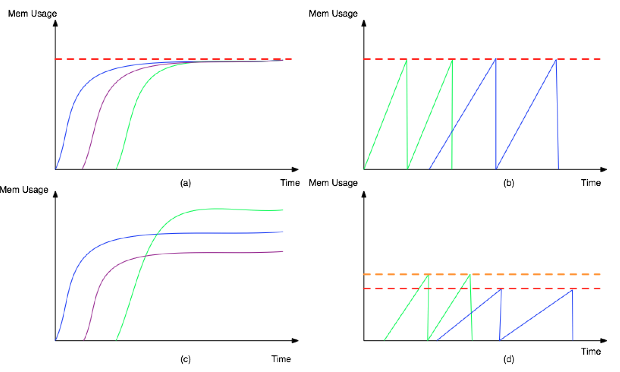
\includegraphics[width=3.0in]{image/workload.png}
    \caption{Four Memory Allocation Behaviors}
    \label{ref:memory_allocation}
\end{figure}

As shown in Figure 9(a), the X-axis red dotted line means the setting for the threshold. All the mappers have the same threshold, and will keep adding data to arraylist until it fills full up of the threshold. In this memory behavior, if the threshold is larger than the JVM maximum heap size setting, the mapper will fail and restart a new attempt with the same threshold. But mappers will start in different time as there is limit on maximum running map task slots in tasktracker. We call this behavior "Same Threshold without Clearance".

As shown in Figure 9(b), the same with the memory behaviro shown in Figure 9(a), all the map tasks have the same memory usage threshold. But the difference is that after each map task full fills its own array to threshold, it will clear all the data in the array which clears the array memory usage to 0, and then start to put data into array list again with exponential increasing speed. We call this behavior "Same Threshold with Clearance".

As shown in Figure 9(c), we can see from the line that there are different thresholds for each map task. This is the setting with the random ratio flag. The random threshold will be calculated when map task starts, and also when it fails and retries. In this case, when some of the map tasks fails due to hold large amount of data, there is chance that it can run without any problems as when it retries the theshold is much smaller than the maximum usage. We call this behavior "Random Threshold without Clearance".

We call the last one shown in Figure 9(d) "Random Threshold with Clearance". It combines the behaviors both from Figure 9(b) and Figure (c).  Every map task has its own threshold, when the data it holds reaches its own threshold, map task will clear the data in the array and then start to put data into array again until it reaches threshold and then clear data again.



\subsection{Experiment Result}

\subsubsection{JVM Heap Size Error}
In default setting of Hadoop, without setting the parameter "mapred.child.java.opt", a default setting with "-Xmx200M" will be transferred to tasktracker to use when start a child JVM for tasks. A naive Hadoop users will never modify these configurations and maybe don't even know hadoop can be configured.
With default settings, Tasktracker will disable the TaskMemoryManagement Thread, so the only reason why the error message shows "Java Heap Size Error" is map task JVM use java heap to restore too much data, which is larger than the set 200MB.
We test with this setting of Hadoop with the customized wordcount described in section 4.1 which has four different types of memory behavior. Using Memmetric we monitor the memory behavior acted as we expected.

\begin{figure}[ht]
  \centering
    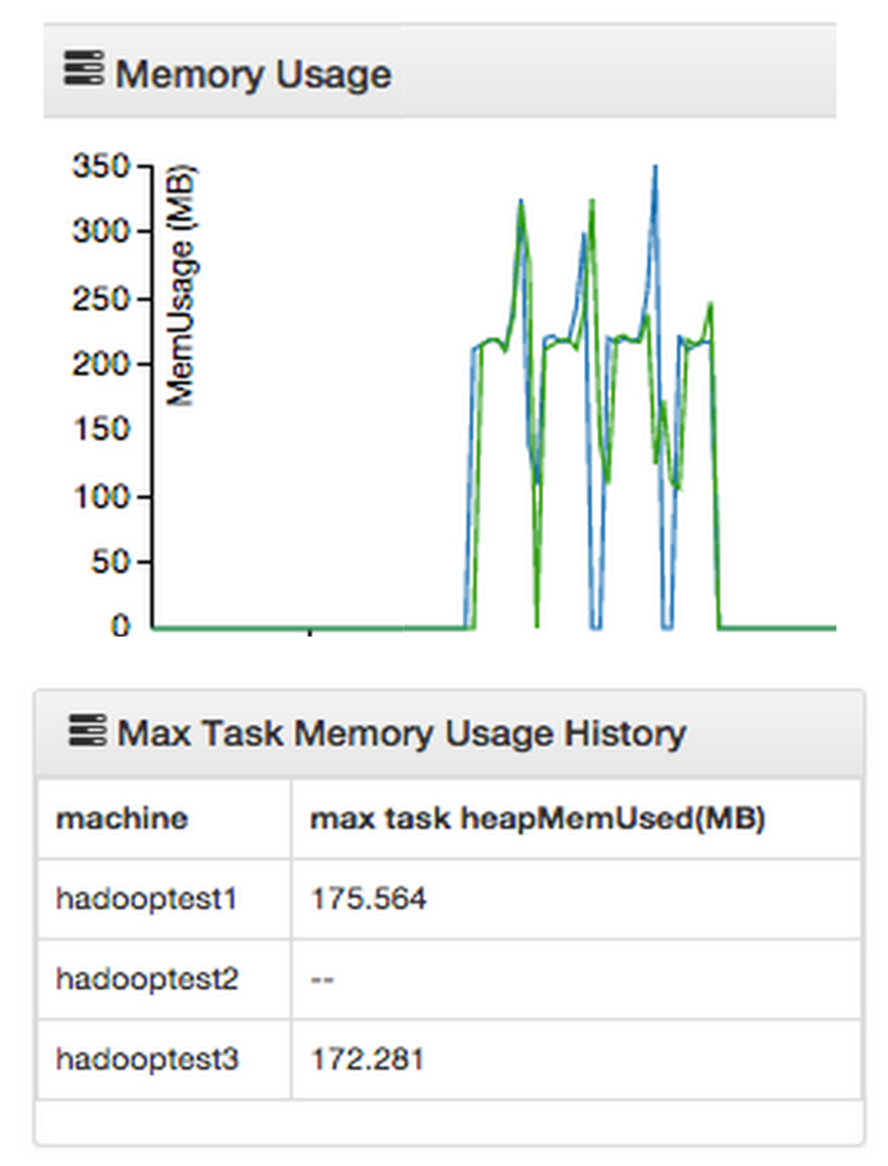
\includegraphics[width=2.1in]{image/test1a.png}
    \caption{Memory Usage under Same Threshold without Clearance}
    \label{ref:memory_allocation}
\end{figure}

In Figure 11

\begin{figure}[ht]
  \centering
    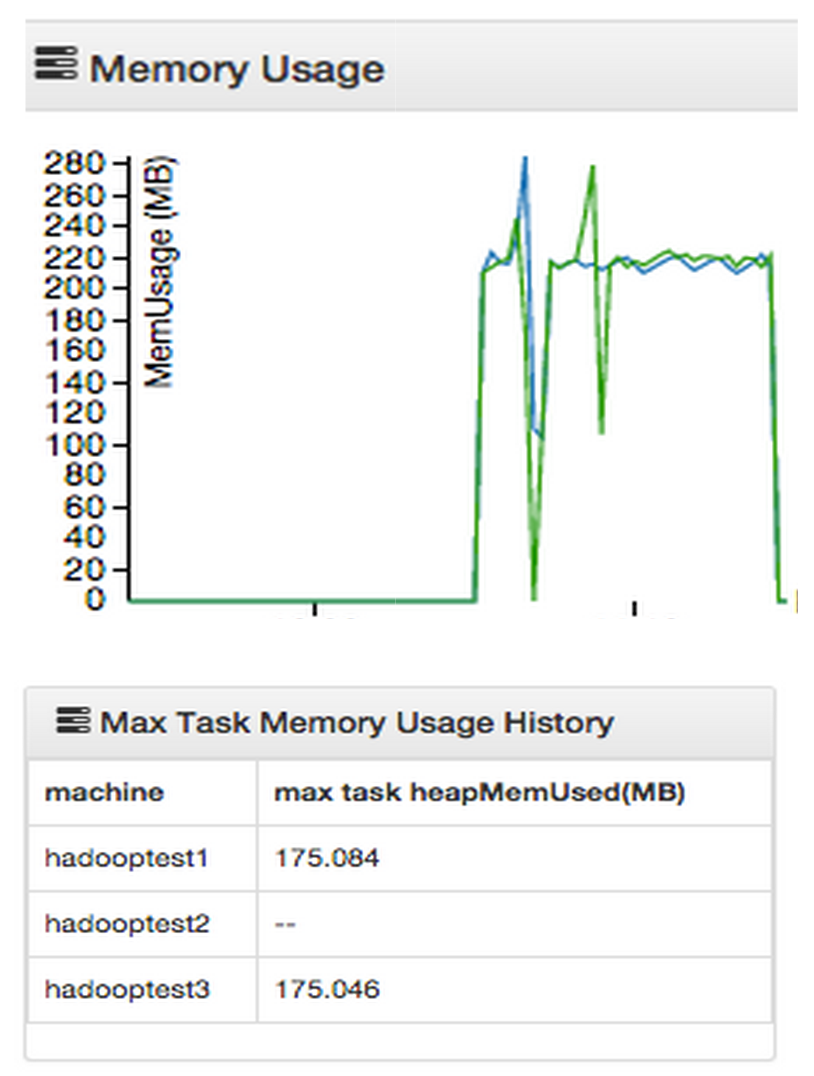
\includegraphics[width=2.1in]{image/test1b.png}
    \caption{Memory Usage under Random Threshold without Clearance}
    \label{ref:memory_allocation}
\end{figure}

\begin{figure}[ht]
  \centering
    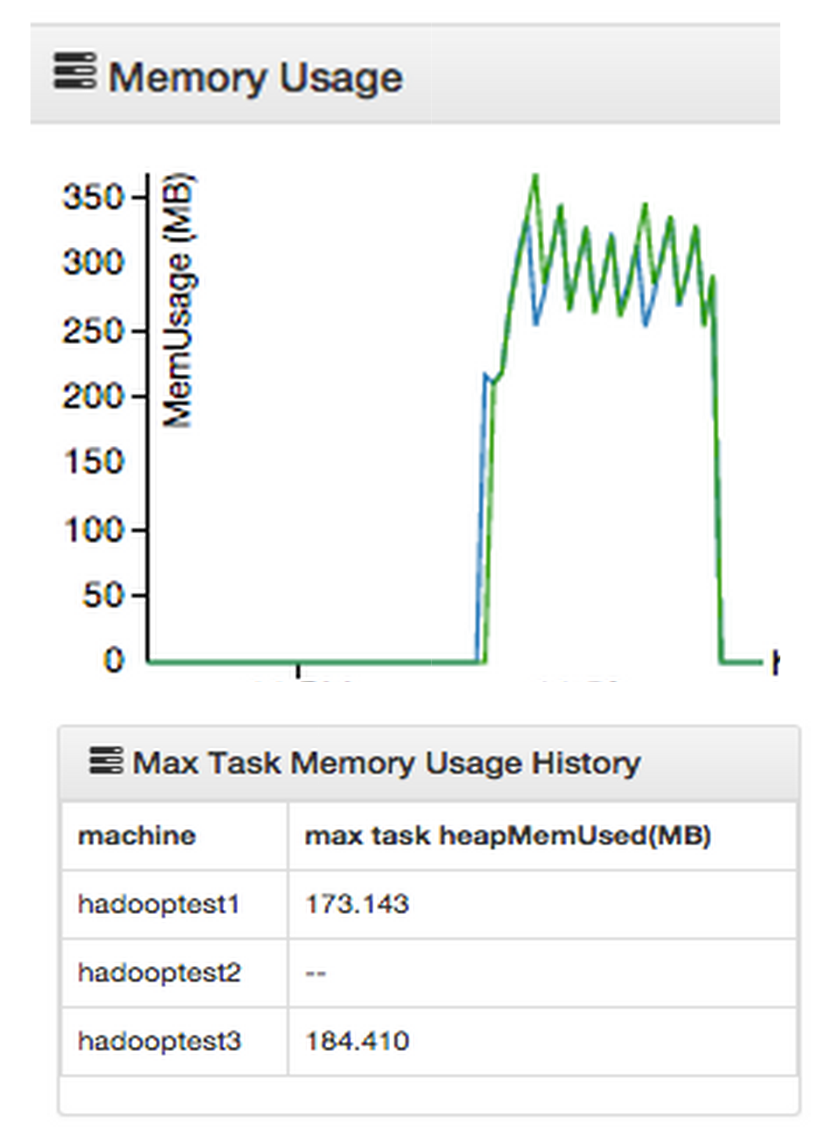
\includegraphics[width=2.1in]{image/test1c.png}
    \caption{Memory Usage under Same Threshold with Clearance}
    \label{ref:memory_allocation}
\end{figure}

\begin{figure}[ht]
  \centering
    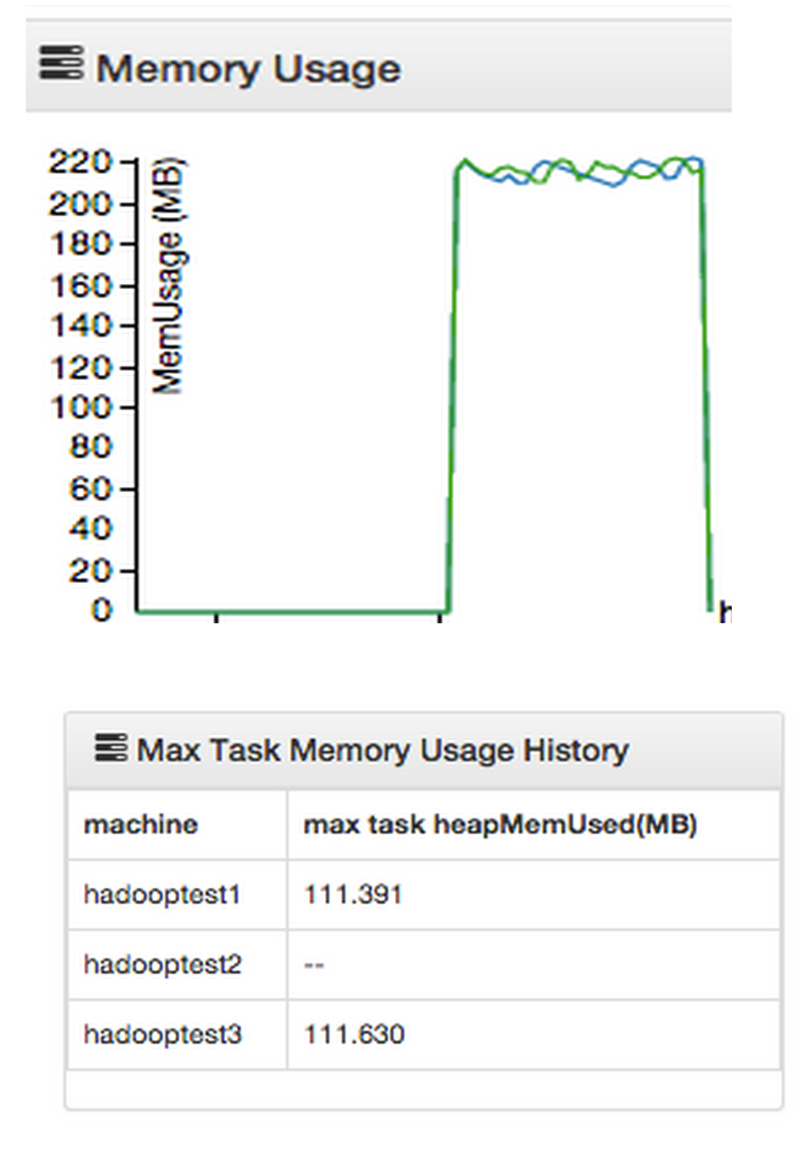
\includegraphics[width=2.1in]{image/test1d.png}
    \caption{Memory Usage under Random Threshold with Clearance}
    \label{ref:memory_allocation}
\end{figure}

\subsubsection{TaskMemoryManagerThread Enabled}
When the parameters are tuned in the configuration file, TaskTrackerManager is enabled. The configuration in this experiment is configured as following.
\begin{align*}
&{\bf mapred.child.java.opts = -Xmx700m}\\
&{\bf mapred.cluster.map.memory.mb = 150}\\
&{\bf mapred.cluster.reduce.memory.mb = 150}\\
&{\bf mapred.cluster.max.map.memory.mb = 200}\\
&{\bf mapred.cluster.max.reduce.memory.mb = 200}\\
&{\bf mapred.job.map.memory.mb = 150}\\
&{\bf mapred.job.reduce.memory.mb = 150}\\
&{\bf mapred.tasktracker.map.tasks.maximum = 2}\\
&{\bf mapred.tasktracker.reduce.tasks.maximum = 1}\\
\end{align*}

When we run this experiment, the 
\par
The reason that this experiment fails is because that the parameters set in this way control the virtual memory usage in the nodes, while Ganglia merely collects heap memory usage and commit memory usage, which are physical memory usage metrics of each node. 

\subsubsection{Execessive Slots}
In this sector, we modified the settings for the maximum running map/reduce tasks in one slave machine, which is called "map/reduce slot number". We set both the value for map and reduce to 8, and makes the threshold for 300MB. As in our test cluster, each slave machine has only 2GB physical memory, the experiment shows the result how hadoop acts in this case. Note that we also modified the JVM Xmx value to 700MB which avoids the memory failure caused by JVM that has been tested in section 4.2.3. We also use the four types of memory behavior as the test applications. 

\begin{figure}[ht]
  \centering
    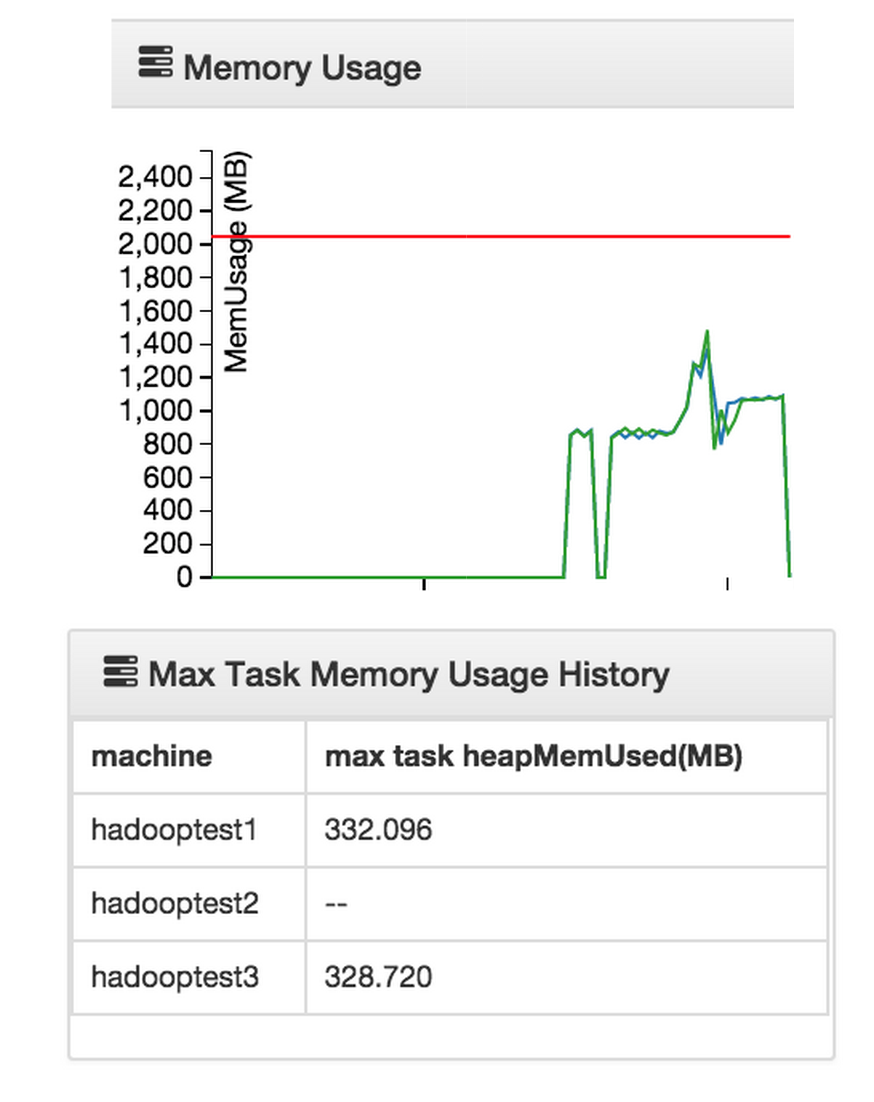
\includegraphics[width=2.1in]{image/test3a.png}
    \caption{Memory Usage under Same Threshold without Clearance}
    \label{ref:test3a}
\end{figure}

In Figure 17, the tested memory behavios is "Same Threshold without Clearance". The whole job failed with error message "there is insufficient memory for the Java Runtime Environment to continue. Native memory allocation (malloc) failed to allocate committing reserved memory." This error makes Child JVM exits with error, as it cannot get enough memory. As we set each mapper's threshold 300MB, and there are 8 mappers running at the same time which will need more than 2GB memory, but the physical space is just 2GB, so in this case all of the mappers will fail as they all cannot get enough memory to continue.

\begin{figure}[ht]
  \centering
    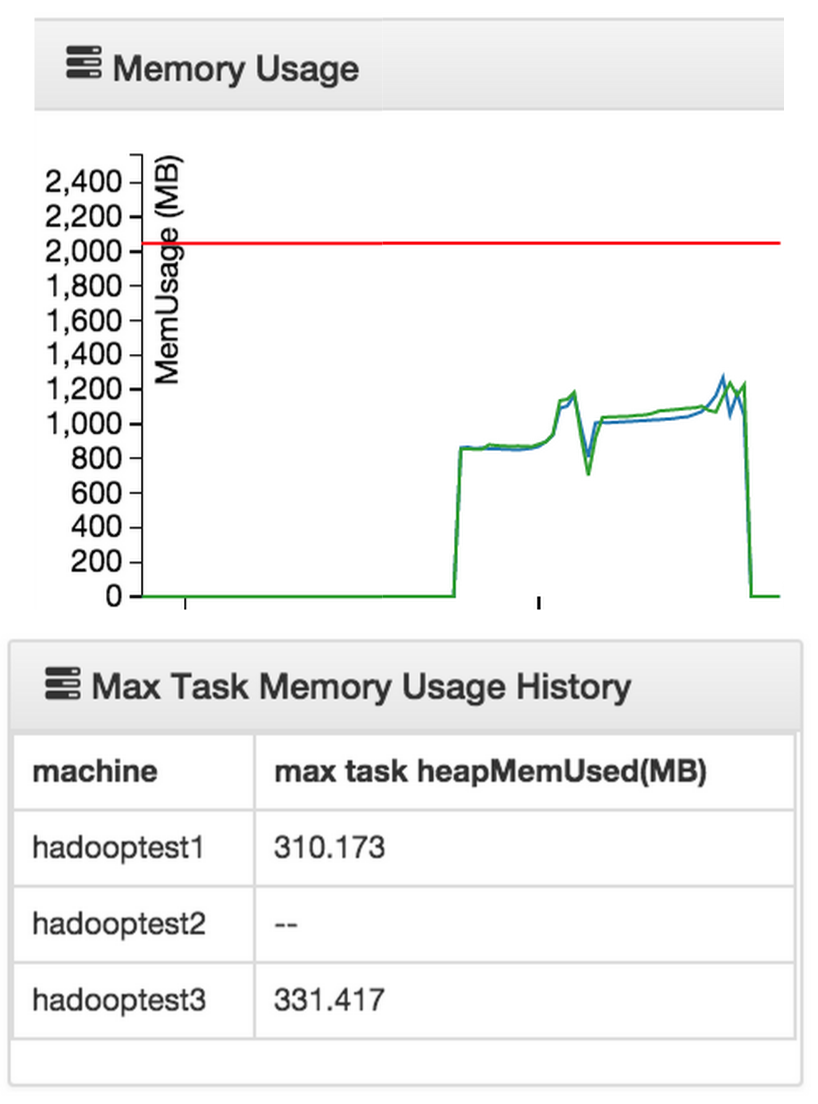
\includegraphics[width=2.1in]{image/test3b.png}
    \caption{Memory Usage under Random Threshold without Clearance}
    \label{ref:test3b}
\end{figure}

In Figure 18, the tested memory behavior is "Random Threshold without Clearance". Even though the threshold is randomized and smaller than 300MB, but some of the mappers still cannot get enough memory for their own threshold, which will cause the child error, and the retry might success, but also might fail. Too many tasks failure will cause the whole job fail, and then it stops.

\begin{figure}[ht]
  \centering
    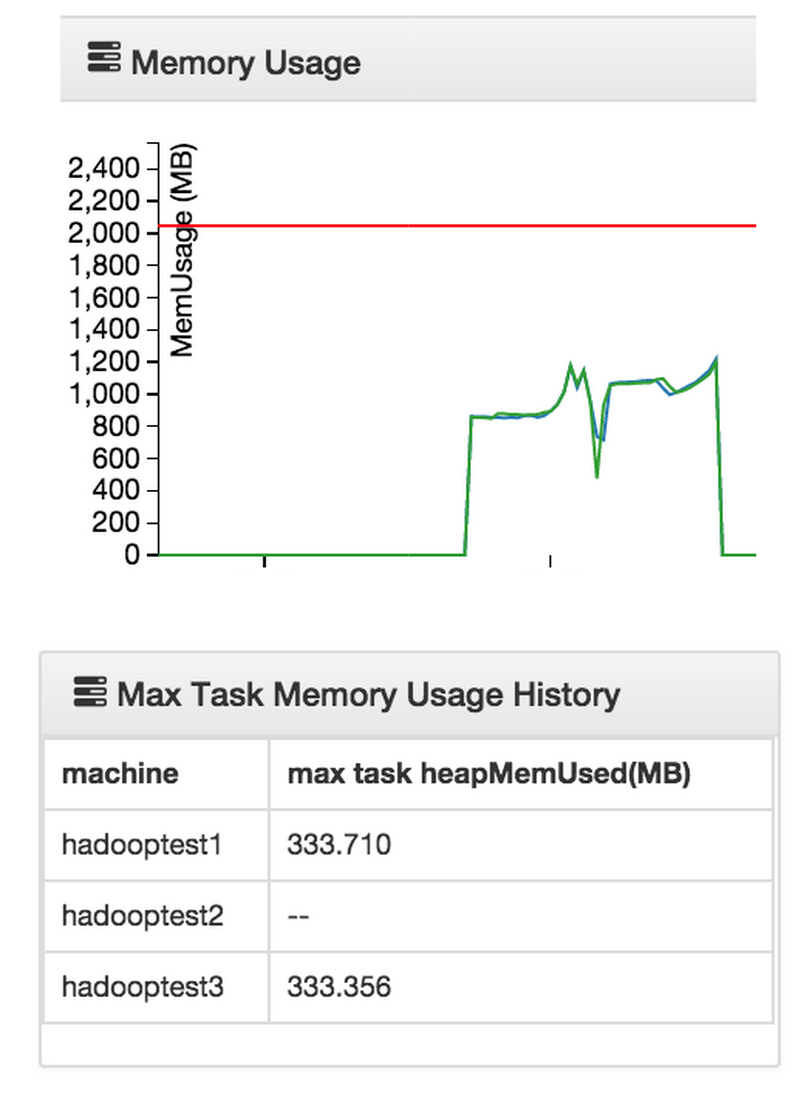
\includegraphics[width=2.1in]{image/test3c.png}
    \caption{Memory Usage under Same Threshold with Clearance}
    \label{ref:test3c}
\end{figure}

In Figure 19, the tested memory behavior is "Same Threshold with Clearance". It still cannot run successfully. As the setting for the threshold is 300MB, none of the maptask can read 300MB and starts to clear the data they hold. Here in this case, it is almost the same with shown in both Figure 17 and Figure 18. As all the mappers are trying to get more data as they can, but the more they want, the easier they fail.

\begin{figure}[ht]
  \centering
    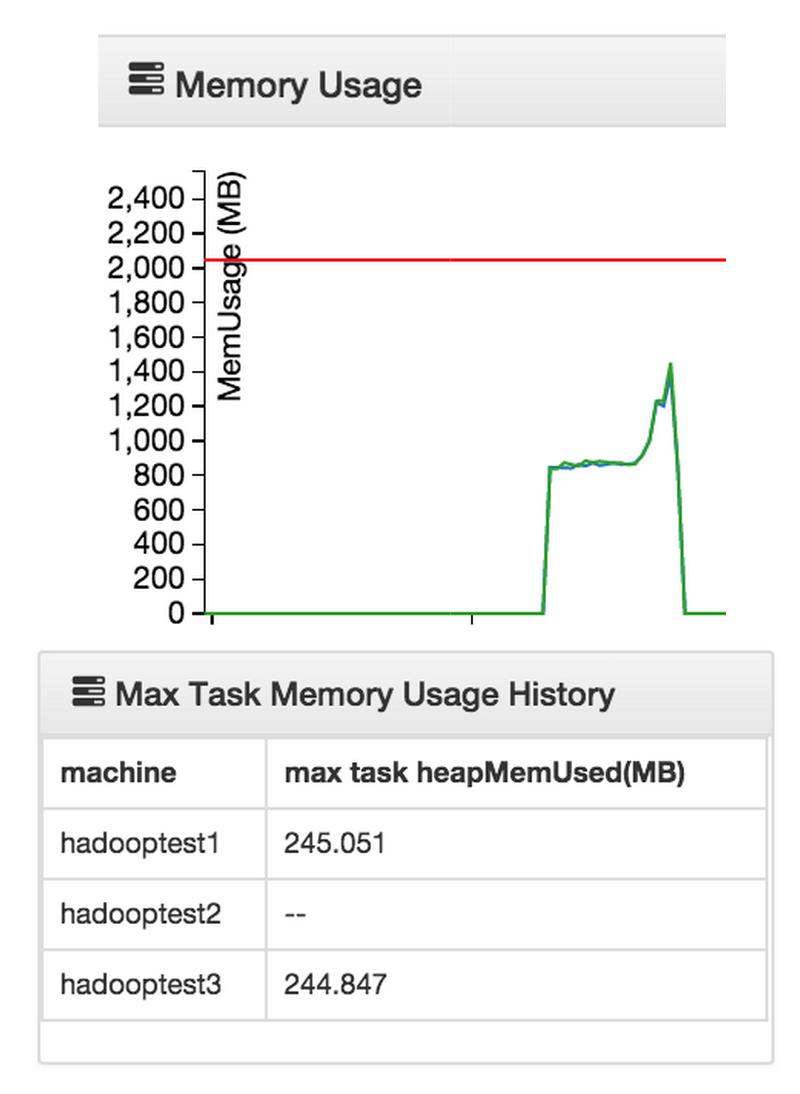
\includegraphics[width=2.1in]{image/test3d.png}
    \caption{Memory Usage under Random Threshold with Clearance}
    \label{ref:test3d}
\end{figure}

In Figure 20, the tested memory behavior is "Random Threshold with Clearance". It still shows failure the same with the former three ones. 

\section{Conclusion}
We built a memory monitor system, Memmetric, for Hadoop 1.2.1 based on Ganglia 3.6.0, which provides users with both real-time and historical monitoring on memory usages to find implicit memory bugs in their Hadoop jobs and to revise their Hadoop cluster parameter settings. 

We found that there is a bug in the connector (GangliaSink31.java) between Hadoop and Ganglia. We fixed it the bug in the new version connector (GangliaSink32.java) to make Ganglia can receive task level metric information.

Besides, We also found that Ganglia is not suitable for task level monitoring inherently. We added Ganglia filter to remove finished job metrics to avoid duplicated memory usage accounting.

Moreover, We designed a set of workload Hadoop jobs to reproduce and study three different types of memory failures: Java Heap Size Failure, TaskMemoryManagerThread Failure, and Excessive Slots Failure. We found that Memmetric can observe Java Heap Size Failure and Excessive Slots Failure, but cannot see TaskMemoryManagerThread Failure, because Hadoop JVM metric does not report virtual memory usage.


\bibliographystyle{plain}
\bibliography{references-bibtex}
\end{document}

